\chapter{Практическая Часть}
В данной части представлен листинг и результат работы программы.
\section{Листинг программы}
\begin{lstlisting}
function lab_2()
   X = [11.89,9.60,9.29,10.06,9.50,8.93,9.58,6.81,8.69,9.62,...
        9.01,10.59,10.50,11.53,9.94,8.84,8.91,6.90,9.76,7.09,...
        11.29,11.25,10.84,10.76,7.42,8.49,10.10,8.79,11.87,...
        8.77,9.43,12.41,9.75,8.53,9.72,9.45,7.20,9.23,8.93,...
        9.15,10.19,9.57,11.09,9.97,8.81,10.73,9.57,8.53,9.21,...
        10.08,9.10,11.03,10.10,9.47,9.72,9.60,8.21,7.78,10.21,...
        8.99,9.14,8.60,9.14,10.95,9.33,9.98,9.09,10.35,8.61,...
        9.35,10.04,7.85,9.64,9.99,9.65,10.89,9.08,8.60,7.56,...
        9.27,10.33,10.09,8.51,9.86,9.24,9.63,8.67,8.85,11.57,...
        9.85,9.27,9.69,10.90,8.84,11.10,8.19,9.26,9.93,10.15,...
        8.42,9.36,9.93,9.11,9.07,7.21,8.22,9.08,8.88,8.71,...
        9.93,12.04,10.41,10.80,7.17,9.00,9.46,10.42,10.43,8.38,9.01];

    gamma = 0.9;

    n = length(X);

    q = mean(X);

    S2 = var(X);

    M_low = find_m_low(n, q, S2, gamma);
    M_high = find_m_high(n, q, S2, gamma);
    S2_low = find_S2_low(n, S2, gamma);
    S2_high = find_S2_high(n, S2, gamma);
\end{lstlisting}

\newpage
\begin{lstlisting}
    M_array = zeros(1, n);
    S2_array = zeros(1, n);
    M_low_array = zeros(1, n);
    M_high_array = zeros(1, n);
    S2_low_array = zeros(1, n);
    S2_high_array = zeros(1, n);

    M_array(1) = X(1);
    S2_array(1) = 0;
    M_low_array(1) = 0;
    M_high_array(1) = 0;
    S2_low_array(1) = 0;
    S2_high_array(1) = 0;

    for i = 2 : n
        temp_m = mean(X(1:i));
        temp_s2 = var(X(1:i));
        M_array(i) = temp_m;
        S2_array(i) = temp_s2;
        M_low_array(i) = find_m_low(i, temp_m, temp_s2, gamma);
        M_high_array(i) = find_m_high(i, temp_m, temp_s2, gamma);
        S2_low_array(i) = find_S2_low(i, temp_s2, gamma);
        S2_high_array(i) = find_S2_high(i, temp_s2, gamma);
    end
\end{lstlisting}
\newpage
\begin{lstlisting}
 plot(1 : n, [(zeros(1, n) + q)', M_array', M_high_array',
M_low_array']);
    xlabel('n');
    ylabel('y');
    xlim([1, n]);

    figure;

    min_n = 6;
    plot(min_n : n, [(zeros(1, n - min_n + 1) + S2)', S2_array(min_n:end)',
S2_high_array(min_n:end)', S2_low_array(min_n:end)']);
    xlabel('n');
    ylabel('z');
    xlim([min_n, n]);
end

function M_low = find_m_low(N, M, S2, gamma)
    M_low = M - sqrt(S2) * tinv((1 + gamma) / 2, N - 1) / sqrt(N);
end

function M_high = find_m_high(N, M, S2, gamma)
    M_high = M + sqrt(S2) * tinv((1 + gamma) / 2, N - 1) / sqrt(N);
end

function S2_low = find_S2_low(N, S2, gamma)
    S2_low = ((N - 1) * S2) / chi2inv((1 + gamma) / 2, N - 1);
end

function S2_high = find_S2_high(N, S2, gamma)
    S2_high = ((N - 1) * S2) / chi2inv((1 - gamma) / 2, N - 1);
end
\end{lstlisting}

\section{Результаты работы программы}

\begin{equation*}
    \begin{split}
        &\hat{\mu} = 9.4872\\
        &S^2 = 1.2173\\
        &\underline{\mu} = 9.3202\\
        &\overline{\mu} = 9.6541\\
        &\underline{\sigma^2} = 0.9959\\
        &\overline{\sigma^2} = 1.5279\\
    \end{split}
\end{equation*}
\newpage

\section{Графики}
Построение на координатной плоскости $O_{yn}$ прямой $y=\hat{\mu}(\vec{x}_N)$, а также графиков функций $y=\hat{\mu}(\vec{x}_n)$, $y=\underline{\mu}(\vec{x}_n)$ и $\overline{\mu}(\vec{x}_n)$ как функций объема $n$ выборки, где $n$ изменяется от 1 до $N$;
\begin{figure}[h!]
    \centering
    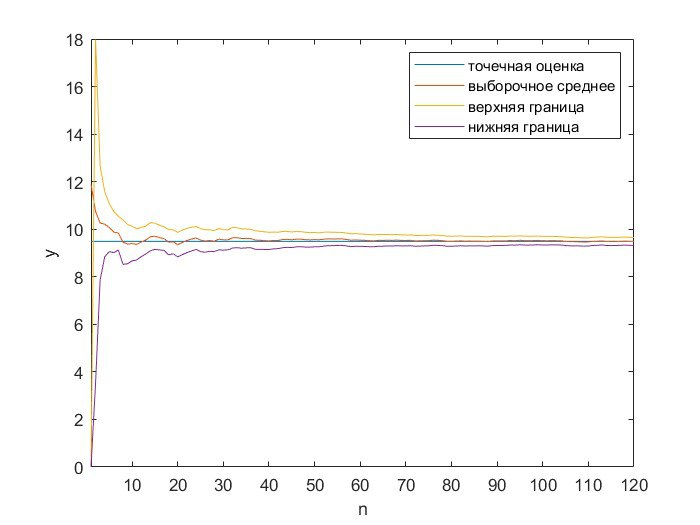
\includegraphics[scale=0.7]{images/2.jpg}
    \caption{График для $\mu$}
\end{figure}
\newpage
Построение на другой координатной плоскости $O_{zn}$ прямой $z=S^2(\vec{x}_n)$, а также графиков функций $z=S^2(\vec{x}_N)$, $z=\underline{\sigma^2}(\vec{x}_n)$ и $\overline{\sigma^2}(\vec{x}_n)$ как функций объема $n$ выборки, где $n$ изменяется от 1 до $N$.
\begin{figure}[h!]
    \centering
    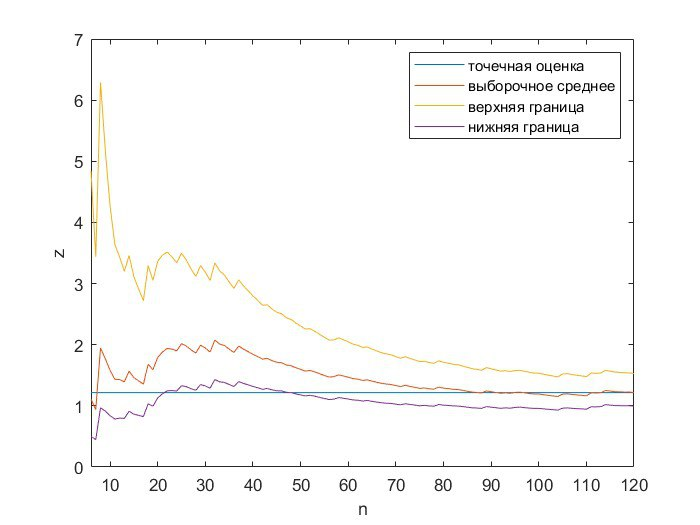
\includegraphics[scale=0.7]{images/1.jpg}
    \caption{График для $\sigma$}
\end{figure}